%!TEX root = these.tex

\chapter[Exploration interactive de données moléculaire en immersion]{Naviguer et visualiser de façon naturelle et immersive}
\label{Sec:CantorDigitalis}
\minitoc
\cleardoublepage

Etape explicite de la boucle de biologie structurale (voir Figure \ref{Fig:schema_seq_bio_struct}), la visualisation de modèles 3d de protéines ou de complexes moléculaires permet à l'expert d'extraire de nombreuses informations de façon intuitive et rapide. Le rôle de la visualisation moléculaire pour communiquer et comprendre la biologie moléculaire a été mise en avant récemment \cite{}.
Nous avons cité plusieurs techniques de visualisation moléculaire dans la section \ref{visu_molecular} permettant de mettre en avant des informations structurelles ou physico-chimiques d'un simple coup d'oeil. Bien que ces informations soient déjà relativement complètes dans des environnements standards, elles peuvent être significativement améliorées par l'ajout de la profondeur dans la perception visuelle des données moléculaires. La RV et les technologies s'y rapportant permettent de rajouter cette 3e dimension grâce aux environnements virtuels (EV) et ainsi permettre une exploration plus naturelle des données.

Cependant, nous avons mis en exergue le frein que constitue la conscience spatiale altérée de l'utilisateur lors de l'exploration de complexes moléculaire dans des conditions immersives. Au-delà de la limitation spatiale que cela impose à l'utilisateur, cette conscience spatiale dégradée entraîne un malaise réduisant significativement la qualité de l'expérience de l'utilisateur. 

Pour répondre à ces problèmes issus directement de la RV, de nombreuses études ont été effectuées. Ces études sont cependant exclusivement réservées pour l'exploration de mondes virtuels écologiques, les études de navigation dans les données abstraites et scientifiques sont quant à elles beaucoup plus rares. 

Nous détaillerons tout d'abord dans ce chapitre notre approche pour répondre à l'évolution des moyens de partager des informations de structure moléculaires dans le monde scientifique. Nous analyserons ensuite les méthodes de navigation dans des scènes écologiques pour identifier les progrès à réaliser dans les scènes de données abstraites. Finalement nous présenterons nos développements et apport pour répondre au besoin de paradigmes de navigation adaptés aux données moléculaires.

\section{Les images stéréoscopiques au service de la visualisation moléculaire}

Nous avons souligné dans le chapitre 2 l'importance que prenait la visualisation et la représentation de structures 3d de molécules pour la compréhension de leur fonctionnement. En plus de permettre d'appréhender leur rôle biologique, la visualisation moléculaire est également un excellent vecteur de communication dans le monde scientifique. Fort de ce constat, nous nous sommes intéressés aux améliorations possibles que nous pourrions apporter aux moyens de communication actuels qu'offre la visualisation moléculaire. Ces derniers se concentrent exclusivement autour de l'échange de représentations graphiques générés par un certain nombre de logiciels experts comme PyMol, VMD ou YASARA pour ne citer qu'eux. Un rendu en deux dimensions d'une vue sur une partie ou l'ensemble d'une molécule permet, avec ou sans légendes appropriées, permet de rendre compte d'un phénomène ou d'une singularité structurelle précise. Si cette singularité est structurelle, elle est par définition 3d et pourrait donc être rendue de façon plus précise par un rendu 3d.

\subsection{L'évolution des méthodes de communication du monde scientifique}

Les moyens de communication scientifique se sont, en parallèle des moyens de communication standards, développés sur les appareils mobiles type smartphone et tablettes. Les journaux physiques et papiers sont de plus en plus rares au sein des labos et la grande majorité des articles scientifiques sont numérisés et accessibles en ligne. Le support a quelque peu évolué et une publication d'un article scientifique, en ligne ou non, suit les mêmes standards de format, majoritairement PDF contenant du texte et des images 2d. Quelques évolutions notoires sont apparues afin d'enrichir les contenus et les rendre interactifs \cite{attwood2010utopia}. Les structures moléculaires peuvent retrouver une 3e dimension grâce à plusieurs méthodes \cite{kumar2008grasping,raush2009new} qui dépendant cependant de pré-requis logiciels minimums pour être complètement fonctionnels ou requièrent des programmes spécifiques (comme la version 3d améliorée d'Adobe Acrobat reader\footnote{\url{http://get.adobe.com/reader/}} ou les plugins spécifiques comme le navigateur ICM\footnote{\url{http://www.molsoft.com/icm_browser.html}}).

En 1994, Green présenta le concept de <<stereoimages>> \cite{green_stereoimages_1994} pour les structures moléculaires. Basées sur la simple décomposition en deux vues, une pour l'oeil droit et une pour l'oeil gauche, de la représentation d'une molécule, elle permet d'avoir une perception 3d de la structure de façon simple et rapide. Nous avons mis à jour cette proposition à la lumière des nouvelles technologies désormais largement disponibles que sont les smartphones et les tablettes. Ces dispositifs mobiles offrent davantage de possibilités pour afficher du contenu scientifique et interagir avec lui facilement et de façon esthétique. Il semble ainsi qu'un décalage dans les habitudes de lecture d'articles scientifiques se fasse. Les éditeurs scientifiques ont d'ailleurs rapidement commencer à publier sur les périphériques mobiles: Cell Press\footnote{\url{http://www.cell.com/journalreader}}, ACS\footnote{\url{http://pubs.acs.org/page/tools/acsmobile/index.html}}, Nature Publishing\footnote{\url{http://www.nature.com/mobileapps}}, Science\footnote{\url{http://content.aaas.org/mobile}} ou PloS\footnote{\url{blogs.plos.org/everyone/2010/09/16/plos-reader-2-0/}} fournissent des application mobiles dédiées pour leurs publications. De la même manière, parmi les nombreuses applications dédiées à la procrastination, certaines se révèlent avoir une utilité scientifique significative \cite{powell_lab_2012}. On retrouve des applications de visualisation 3d de biomolécules, de visualisation 2d de petites molécules, des applications de calcul de masse molaire ou des applications informatives comme un tableau périodique. On retrouve parmi ces applications mobiles "scientifiques" une simplicité commune et des qualités de graphismes modestes, principalement dues aux puissances graphiques matériellement limitées des périphériques mobiles. Il est ainsi compliqué de permettre un rendu 3d complet d'un complexe moléculaire de taille raisonnable sur ces appareils.

\subsection{DepthMol3d}

Il est cependant possible d'utiliser la puissance graphique, même restreinte, des smartphones/tablettes pour créer une perception 3d améliorée de systèmes moléculaires. C'est le but du développement de notre application, DepthMol3d, basé sur le moteur de jeu Unity3D\footnote{\url{http://unity3d.com/}}. Cette approche offre de nombreuses opportunités pour la recherche, la communication, la discussion et le monde de l'éducation.

Notre approche se place au plus près des techniques d'immersion cognitive qui cherche à jouer sur la réflexion des utilisateurs pour les immerger dans la scène virtuelle représentée. Les aspects 3d sont importants et la perception de l'objet jouera un rôle dans l'immersion mais elle sera naturellement limité par le dispositif et l'absence de stimuli sensoriels autres que visuels. Cependant, c'est l'imagination de l'utilisateur et sa capacité de réflexion qui auront un rôle prépondérant pour son implication.

\subsubsection{Ajouter la 3e dimension à une scène moléculaire}

Notre approche se base sur l'utilisation d'images 2d, beaucoup plus légères que des modèles 3d et permettant un certain degré de personnalisation de la part des utilisateurs. Indépendante de logiciels experts de visualisation, notre méthode ne nécessite qu'un périphérique mobile pour fonctionner et expérimenter l'effet 3d. Un nombre important de visualiseurs moléculaires peuvent être utilisés pour générer du contenu, VMD, Chimera, PyMol ou Yasara ont par exemple été utilisé pour générer plusieurs scènes exemples.

Deux images sont nécessaire pour parvenir à un effet 3d, une image de \textbf{texture} et une \textbf{carte de profondeur} (cf. Figure \ref{Fig:depthmol3d_process}). L'image de \textit{texture} est une capture de la scène 3d moléculaire. La \textit{carte de profondeur} possède elle les informations de profondeur pour l'image de texture à travers un gradient de couleur grise. Ce gradient de gris correspond à la distance entre chaque point de l'objet 3d et l'écran. Plus un objet est distant de la caméra (ou de l'écran d'ordinateur) et plus la couleur est sombre. Une fois que les deux images ont été générées, elles doivent être transférées sur le périphérique mobile où elles sont lues et traitées par notre application. Un navigateur de fichier intégré permet à l'utilisateur de trouver ses images et de les charger. Le principe d'une telle application est de créer un objet 3d à partir de la carte de profondeur dont la surface sera ensuite colorée par la texture associée (\ref{Fig:heightmap_texture_unity}). Avec ces données, l'application crée l'illusion d'une 3e dimension en ajoutant aux objets une sensation d'espace et de profondeur qui s'étend loin derrière l'écran. Cela est rendu possible par les calculs permanents de la direction de vue basée sur l'orientation du périphérique, mesurée par un accéléromètre ou un gyroscope embarqués dans la majorité des périphériques mobiles d'aujourd'hui, amenant à la sensation de regarder à l'intérieur d'une boîte qui s'étendrait derrière la surface d'écran de l'appareil.
Il est possible d'utiliser jusque 4 images (2 fois deux images contenant une carte de profondeur et une texture associée) afin de créer des scènes plus complexes possédant un arrière-plan et un premier-plan. Cette possibilité permet l'ajout d'informations complémentaires qui ne sont généralement pas présent au sein des visualiseur moléculaire d'où les scènes virtuelles sont extraites.
Plusieurs exemples sont fournis avec l'application permettant à l'utilisateur d'appréhender les rendus 3d possibles et d'avoir une première prise en main des possibilités qu'offrent l'application. Les 6 exemples sont illustrés dans la Figure \ref{Fig:depthmol3d_exemple}.

\begin{figure}
\begin{subfigure}{.5\textwidth}
  \centering
  {\includegraphics[width=.75\linewidth]{./figures/ch3/depthmol3d_process}}
    \caption{}
  \label{Fig:pymol_stereo}
  % \hspace{0.3cm}
\end{subfigure}
\begin{subfigure}{.5\textwidth}
  \centering
  {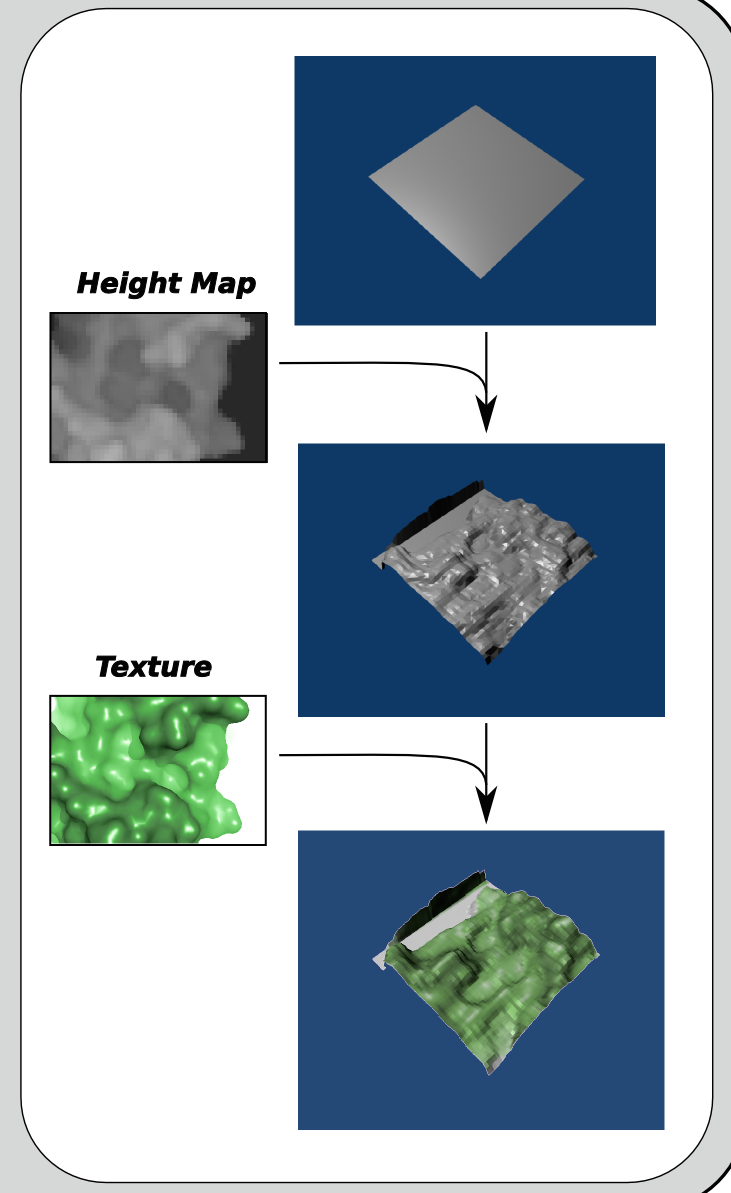
\includegraphics[width=.75\linewidth]{./figures/ch3/heightmap_texture_unity}}
    \caption{}
  \label{Fig:heightmap_texture_unity}
  % \hspace{0.3cm}
\end{subfigure}
\caption{{\it (a) Schéma du fonctionnement de notre application mobile. La première étape consiste à générer une carte de profondeur et une capture d'image de la scène moléculaire que l'on souhaite visualiser. Les deux images sont ensuite combinées au sein de l'application pour créer une perception 3d de la scène initiale.
(b) Le processus d'obtention d'un objet 3d à partir de 2 images. La première étape consiste à analyser la carte de profondeur pixel par pixel et de générer une surface aux dimensions identiques (à un facteur d'échelle près) dont la hauteur de chaque sommet sera corrélée avec le niveau de gris du pixel correspondant.}}
\end{figure}

\begin{figure}
\begin{subfigure}{.5\textwidth}
  \centering
  {\includegraphics[width=.75\linewidth]{./figures/ch3/depthmol3d_exemple}}
    \caption{}
  \label{Fig:depthmol3d_exemple}
  % \hspace{0.3cm}
\end{subfigure}
\begin{subfigure}{.5\textwidth}
  \centering
  {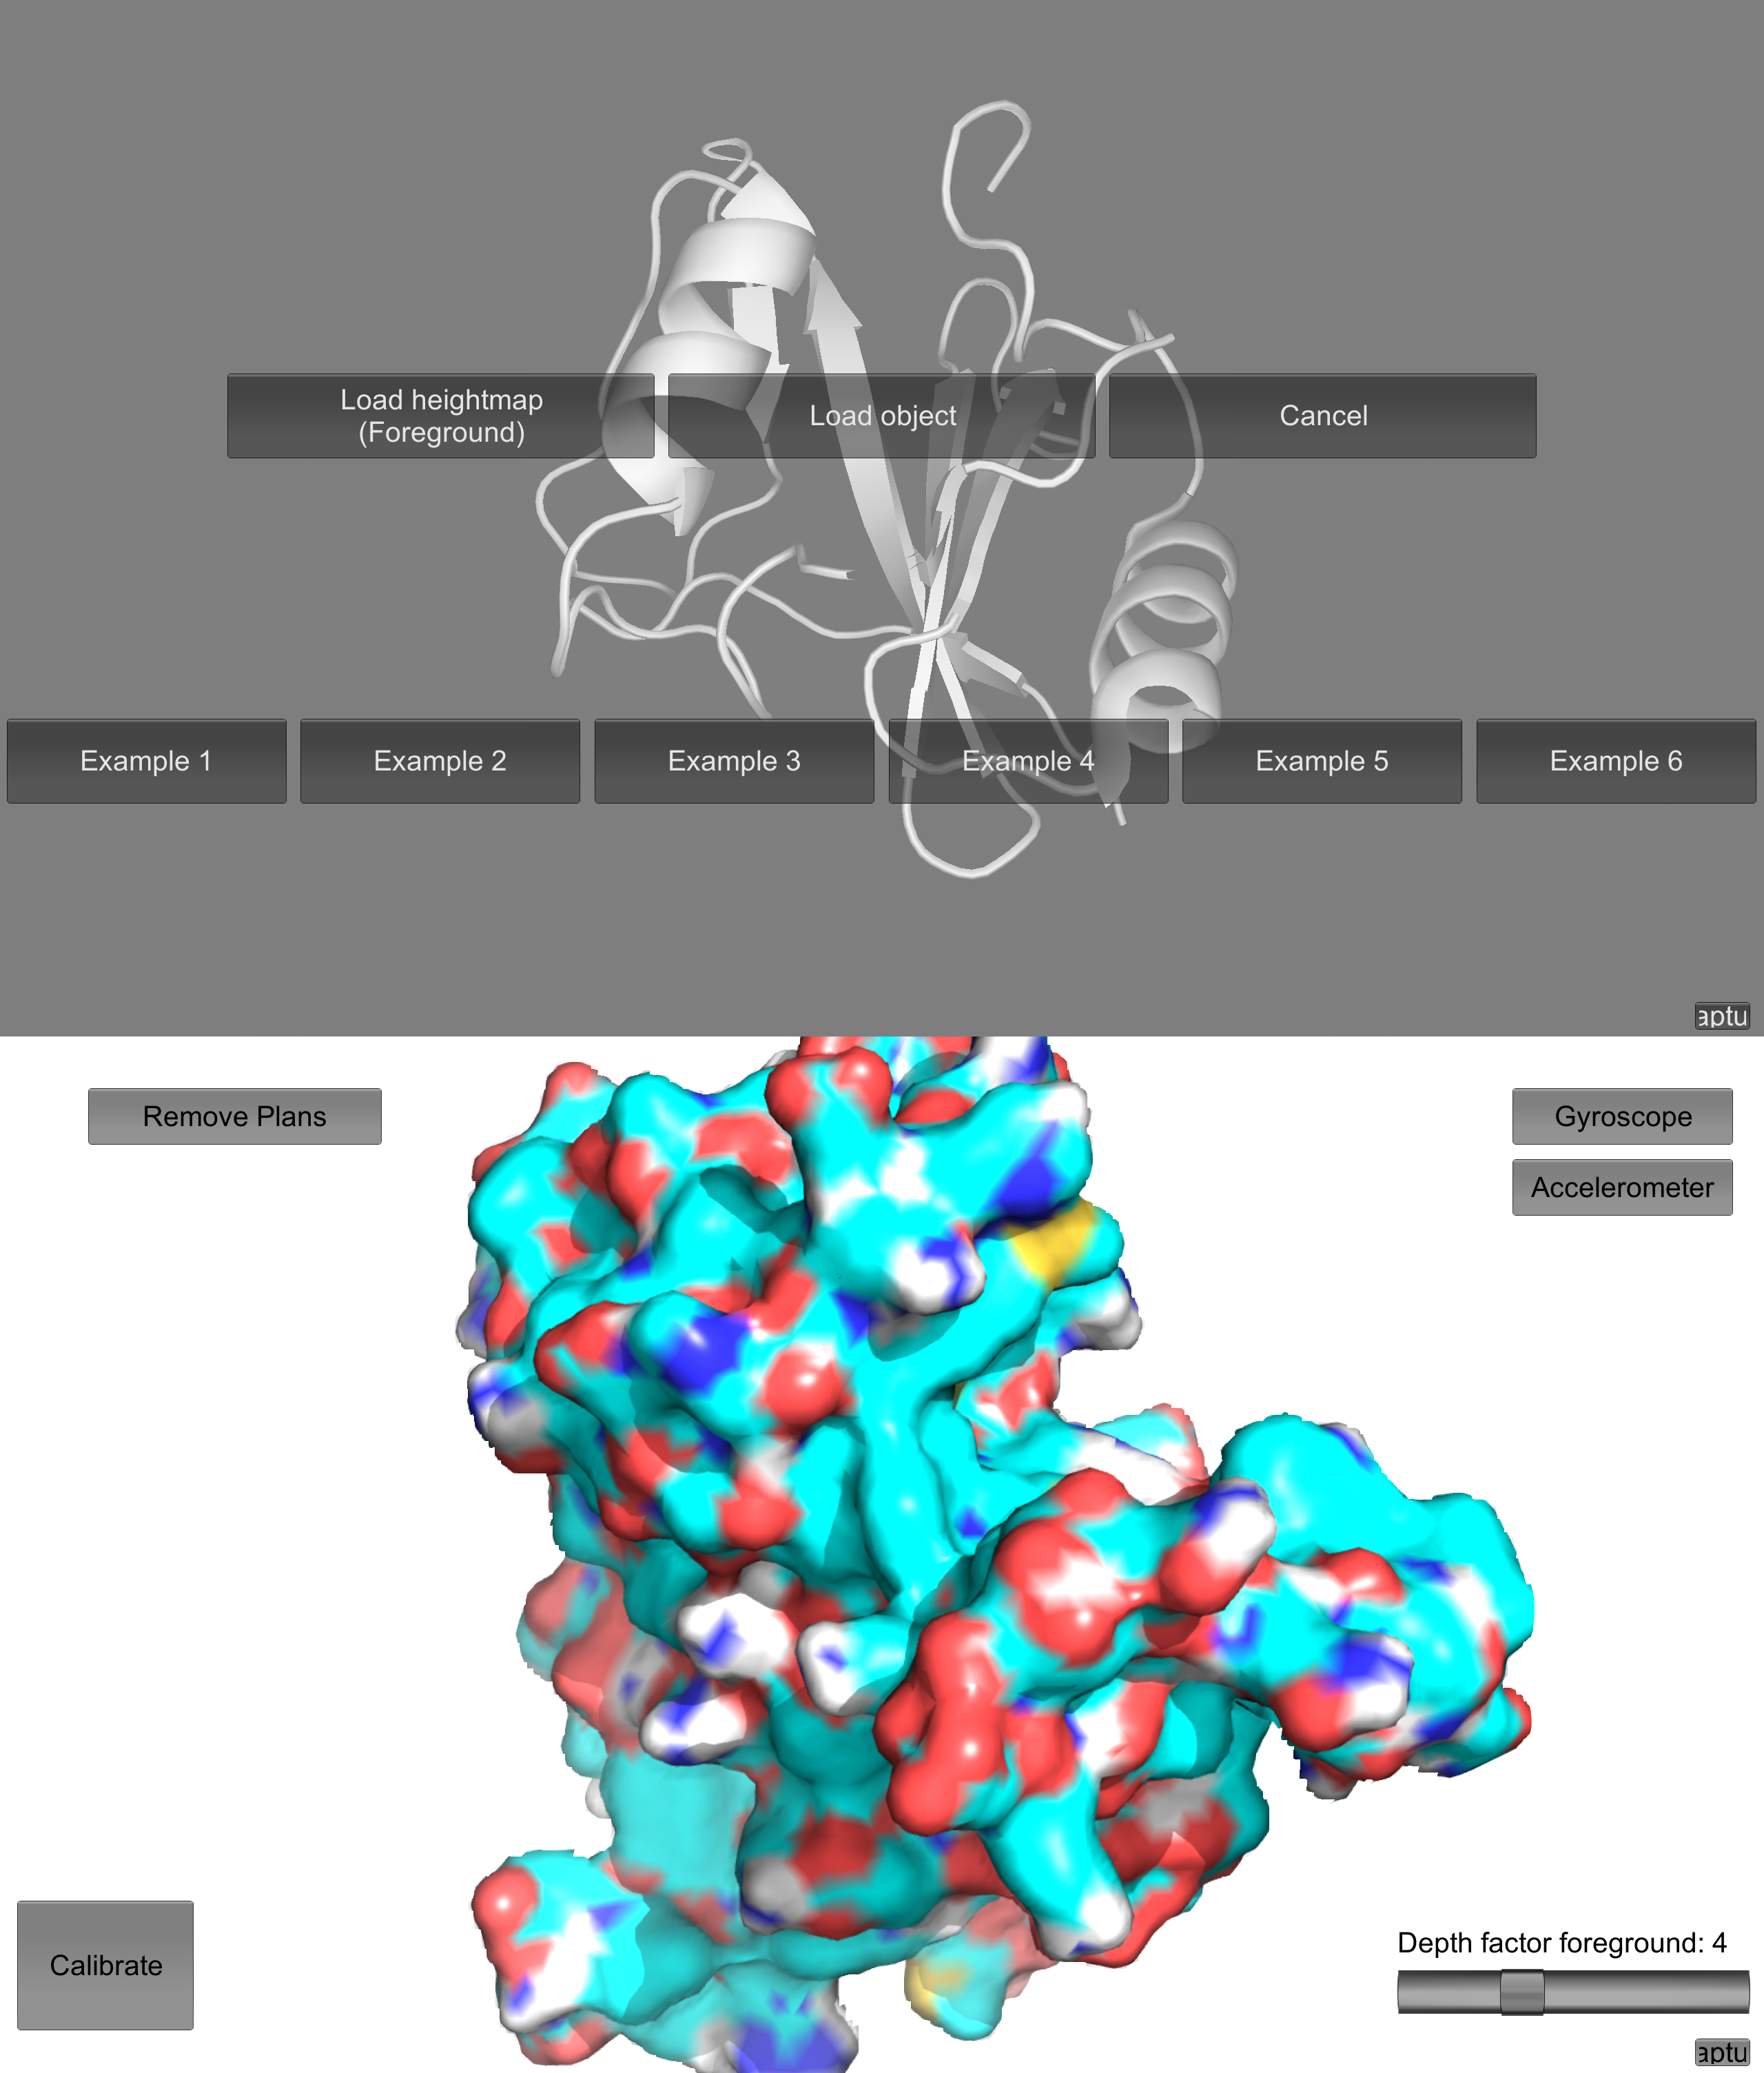
\includegraphics[width=.75\linewidth]{./figures/ch3/depthmol3d_screenshots}}
    \caption{}
  \label{Fig:depthmol3d_screenshots}
  % \hspace{0.3cm}
\end{subfigure}
\caption{{\it (a) Scènes moléculaires proposées par défaut en exemple au sein de l'application.
A. Visualisation d'une poche de liaison à la surface de GLIC (Ligand-Gated Ion Channel), une protéine transmembranaire responsable du passage des ions et des molécules d'eau à travers la membrane cellulaire. Scène extraite de VMD. B. Carte de basse résolution obtenue à partir de cryo-EM pour un filament d'actine. La position de la structure atomique dans l'enveloppe de basse résolution est en premier-plan alors que la carte électromagnétique est présentée en arrière-plan. Visualisation provenant de Chimera C. Couple verticale du modèle de la capside du virus Influenza A exposant la membrane externe et l'intérieur du virus. GraphiteLifeExplorer a été utilisé pour visualiser la coupure. D. Interaction entre une protéine SNARE et une membrane biologique lors d'une dynamique moléculaire (arrière-plan). Un graphe 3d rapportant le taux de courbure de la membrane est présenté en premier-plan. La surface 3d a été générée par Paraview (programme de visualisation scientifique) E. Scènes extraites d'un programme d'animation, MolecularMaya, dédié à la création de films scientifiques pour une audience large. Les scènes extraites mettent en avant deux virus au milieu de villosités à gauche et de multiples virus à droite.
(b) Captures d'écran provenant de l'application DepthMol3D et mettant en avant le menu principal de l'application permettant de charger une image ou un objet 3d (en haut) et une scène 3d type représentant la surface d'une protéine avec les différentes options de paramétrisation (en bas).}}
\end{figure}

\subsubsection{Explorer des modèles 3d de molécules}

Un deuxième mode de visualisation permet d'importer directement des mesh 3d dans DepthMol3d. Avec ce type de données 3d, seul un fichier est nécessaire pour créer une perspective 3d. Après importation, il est possible de manipuler l'objet, de le tourner, le déplacer en avant ou arrière. Cette visualisation se rapproche de ce qui peut se retrouver dans les visualiseurs moléculaires pour périphériques mobiles à ceci près que l'utilisateur aura également la possibilité de changer l'échelle de la molécule et de plonger à l'intérieur. 

Il utilisera alors son périphérique comme une fenêtre sur le monde virtuel, à la manière de ce que proposent de nombreux acteurs de la RV aujourd'hui n'ayant pas franchi le pas de la conception de casques de RV mais fournissant des supports de smartphones (voir section \ref{dispositifs_RV}). Basés sur le gyroscope du périphérique, un simple mouvement de tête permet de regarder une zone différente de la molécule (voir Figure \ref{}). Cette approche est rendue possible par un mode stéréoscopique \textit{side-by-side} intégré au sein de l'application. Il est cependant possible de garder une approche plus simple en orientant le téléphone à la main et en l'utilisant comme une vue adaptative sur un monde virtuel présent tout autour de lui.

\subsubsection{Bilan}

La préparation des images utilisées au sein de l'application est relativement simple et rapide, des tutoriels sont en plus préparés pour aider les utilisateur à effectuer les actions nécessaires. Notre approche est indépendante de la plateforme de visualisation et la majorité des visualiseurs moléculaires permettant de générer des rendus graphiques de structures permettent de générer les images demandées. Il est également possible d'utiliser des outils génériques tels que Povray\footnote{\url{www.povray.com}} ou Paraview\footnote{\url{www.paraview.org}}. La création de vues complexes est rendue possible grâce à la notion d'arrière-plan et de premier-plan permettant ainsi de mettre en valeur certains aspects d'une scène virtuelle où la seule structure ne serait pas assez illustrative d'un phénomène particulier.

La performance de l'application permet son utilisation sur la plupart des smartphones et tablettes Android et iOS de moins de 5 ans et la quasi-intégralité des derniers smartphones/tablettes. DepthMol3D est gratuit et le code source est disponible à la demande.

Les limitations de notre application résident tout d'abord dans la résolution des écrans des périphériques et leurs angles de vue, tout deux limités par rapport aux stations de travail ou aux ordinateurs portables à cause de leur taille. Les cartes de profondeur sont pour le moment limitées à des résolutions assez basses et peuvent faire apparaître des artefacts quand les détails de la scènes sont trop fins. La limitation de la résolution des cartes de profondeur considérées dans l'application est due à la limitation technique du moteur Unity3D qui ne peut gérer des objets 3d de plus de 65536 sommets. Ceci implique donc l'utilisation de cartes de profondeur de 255*255 pixels de résolution au maximum. Il n'existe par contre aucune limitation dans la résolution de la texture tant que celle-ci est aux mêmes dimensions que la carte de profondeur. L'utilisation d'images 2d ne permet pas un contrôle total de l'objet 3d généré et sa manipulation dans l'espace. Notre mode d'importation d'objets 3d permet de pallier en partie cette limitation mais la performance du rendu est moindre, tout autant que la facilité de création de nouvelles structures.


\section{Navigation dans des scènes réalistes ou scientifiques}

Nous avons vu dans le chapitre précédent (voir section \ref{navigation}) que la navigation dans des EV immersifs se caractérisait pas la volonté d'étendre les capacités d'exploration de mondes virtuels malgré les limites physiques imposées par les EV immersifs.

La navigation dans des données de différentes natures a amené la RV à développer différentes techniques de navigation afin de répondre efficacement aux différents contenus et interactions proposés. Ces techniques répondent à différents niveaux de contrôle laissés à l'utilisateur dans sa tâche de navigation et doivent permettre d'assurer une expérience la plus intuitive et confortable qui soit.

Après avoir énoncé les différents niveaux de contrôle existants pour la navigation en EV immersif, nous nous intéresserons aux paradigmes ayant été développés pour répondre à la fois aux scènes virtuelles réalistes, axe majeur d'étude en RV, et également aux scènes que nous appellerons <<abstraites>>, accusant d'un retard plus important.
Nous présenterons finalement notre contribution pour répondre au retard mis en avant pour l'exploration efficace de complexes moléculaires en conditions immersives.

% La navigation dans des environnements virtuels 3d possède un certain degré de similitude avec la navigation dans le réel. La différence principale entre la navigation dans les espaces réel et virtuel se situe au niveau des modes/techniques de navigation qui sont propres à chaque réalité. La navigation est un concept très vaste qui nécessite dans un premier temps une clarification terminologique. Darken et Peterson (2002), spécialistes en cognition spatiale, remarquent qu'une confusion apparaît dans la littérature sur les termes employés. Ainsi, certains auteurs emploient comme synonyme les termes de « navigation », « déplacement » ou encore « exploration ». Ces trois termes sont au centre de la présente recherche d’où l’importance de définir clairement ces mots-clés. 
% La navigation dans des environnements réels ou virtuels se définit à la fois par des composantes \textbf{motrices} et à la fois par des composantes \textbf{cognitives} \cite{bowman_doug_a_3d_2002}.

% \begin{itemize}
% 	\item La composante motrice définit le mouvement/déplacement réel d’un utilisateur dans l’espace. Il existe plusieurs modes ou techniques de déplacement. Bowman (2002) les classe en deux catégories, selon la métaphore employée pour se déplacer dans l’espace virtuel :
% 		\begin{itemize}
% 			\item Les métaphores réelles qui font appel à des comportements réalistes et/ou naturels comme le déplacement en mode « marche », « vol », « à vélo » ou encore « en conduisant ».
% 			\item Les métaphores « virtuelles » où les chercheurs utilisent le potentiel du virtuel pour imaginer et créer des modes de déplacement dans l’espace. Ainsi, ces métaphores permettent de s’extraire des contraintes physiques. Elles demandent par conséquent l’apprentissage de leur fonctionnement. Parmi ces métaphores dites « virtuelles », on peut citer la téléportation (on spécifie les coordonnés de la cible à atteindre) par exemple.
% 		\end{itemize}
% 	\item La composante cognitive ou « wayfinding » est un processus cognitif de définition d’un chemin à travers un environnement. Le « wayfinding » a pour rôle de se construire une « carte cognitive »[26] de l’espace visité et de l’utiliser.
% \end{itemize}

% Dans un environnement virtuel, les utilisateurs peuvent disposer de plusieurs objectifs ou tâches à effectuer. Trois tâches de navigation ont été identifiées par Darken et Sibert \cite{darken1996navigating} de façon générique alors que Van dam et al. \cite{van_dam_immersive_2000} ainsi que Bowman \cite{bowman_doug_a_3d_2002} en proposent une quatrième prenant tout son sens dans le cadre de la navigation pour la visualisation scientifique:

% \begin{enumerate}
% 	\item  L'\textbf{exploration} c’est-à-dire une navigation sans cible explicite à atteindre. Le but étant uniquement de connaître et comprendre le nouvel environnement exploré. L’exploration peut aussi être psychologiquement active si le sujet doit suivre des indications. Dans le cas contraire, l’exploration est dite psychologiquement passive.
% 	\item La \textbf{recherche d'une cible inconnue} où le sujet cherche une cible/destination particulière mais ne connaît pas la position de celle-ci.
% 	\item La \textbf{recherche d'une cible dont la position est connue} (à un certain degré). La tâche/objectif étant de retrouver la cible.
% 	\item La \textbf{manoeuvre} consiste en des mouvements courts et précis destinés à positionner ou orienter l'utilisateur de façon optimale pour effectuer une tâche.
% \end{enumerate}


% La dissociation entre les distances pouvant être parcourues dans un monde virtuel et les contraintes dimensionnelles des dispositifs immersifs a rapidement obligé les experts en RV de mettre au point des méthodes de navigation adaptées. Ces nouvelles méthodes ne répondent pas seulement au besoin de changement d'échelle entre l'espace réel d'interaction et l'espace virtuel de navigation, elles doivent également prendre en compte la contre-productivité d'une navigation libre menant souvent à une perte de repères spatiaux. C'est par exemple le cas d'exploration immersive de structures bornées et courbées par des couloirs ou des parois que, sans retour haptique performant, l'utilisateur ne pourra que difficilement éviter. 

% Cette perte de repères spatiaux n'est pas le seul fait de paradigmes de navigation offrant trop de liberté, elle sera également accentuée par l'abstraction des données observées. Alors que la navigation au sein d'une ville ou d'une pièce peut permettre, par l'hétérogénéité des objets/bâtiments/personnages s'y trouvant, de garder une conscience de sa position et de son orientation suffisante, la navigation dans une scène possédant une majorité d'informations abstraites et/ou non orientées diminuera cette capacité à savoir à chaque instant sa position par rapport au contenu et au monde virtuel. Les degrés de liberté de l'utilisateur pour naviguer dans sa scène virtuelle sont également un facteur pouvant compromettre sa bonne conscience spatiale. Alors que les scènes réalistes vont souvent induire une navigation avec 2 degrés de liberté parallèlement au sol virtuel, les scènes possédant des données abstraites peuvent aisément permettre une navigation en 3 dimensions dans l'ensemble du volume composant la scène virtuelle. Cela influe également l'orientation de l'utilisateur qui gardera souvent un point de vue parallèle à l'horizontale de la scène dans le cas de scènes réalistes, point de vue qui n'aura pas les mêmes contraintes lors de la navigation avec 3 degrés de liberté.

% La réduction ou l'absence de repères spatiaux n'a pas seulement une conséquence sur le fait qu'un utilisateur puisse se sentir perdu au milieu d'une scène virtuelle. Elles peut également déclencher ou favoriser l'apparition d'un malaise, communément appelé \textit{cybersickness}. 

% \subsection{Malaise virtuel ou \textit{cybersickness}}

% Le \textit{cybersickness} peut s'apparenter au mal des transports, transposé aux mondes virtuels, et se caractérisant par plusieurs effets néfastes pour l'utilisateur. En plus de simples sensations d'inconfort, on retrouve comme symptômes de la fatigue excessive, des vertiges, des maux de tête ou des nausées, tous très négatifs pour l'expérience de l'utilisateur \cite{kolasinski1995simulator,laviola_jr_discussion_2000}. Ce malaise empêche donc clairement l'efficacité de l'utilisateur pour effectuer ses tâches expertes et induit également un phénomène de "méfiance" vis-à-vis du dispositif immersif pouvant entraîner une volonté de ne pas reproduire l'expérience. Ce phénomène fut donc étudié de près afin d'en identifier les causes et d'en trouver des solutions. Les causes principales ressorties des expériences de RV menées dans le but d'induire ce phénomène passent presque exclusivement par la dissociation des canaux perceptifs du corps humain. Le découplage des informations fournies par canal visuel avec celles du système vestibulaire est particulièrement problématique. La différence de la nature des informations provenant des différents systèmes sensoriels par rapport à l'expérience usuelle de l'utilisateur a donc une chance importante d'induire ce malaise chez certaines personnes\cite{reason1975motion}.

% Typiquement, une scène virtuelle impliquant un déplacement non contrôlé de l'utilisateur et dont les paramètres de vitesse, d'accélération et de rotations ne sont pas finement paramétrés, entraînera dans beaucoup de cas un malaise de l'utilisateur. Ces situations de déplacements incontrôlés sont également responsables du mal des transports. L'absence d'implication d'un usager sur son moyen de transport, quand celui-ci possède une trajectoire et une vitesse variant de façon aléatoire, peut aussi induire un malaise. Ce phénomène de retrouve de façon négligeable lors du visionnage d'un film ou d'un contenu vidéo impliquant les mêmes déplacements mais sur un support 2d. L'immersion joue donc un rôle très important dans ce phénomène et la fidélité de restitution d'une scène réaliste impliquera souvent une probabilité de malaise plus important. Un exemple récent du rôle de l'immersion et de la stéréoscopie comme facteur de \textit{cybersickness} est le film "The Walk"\footnote{\url{https://en.wikipedia.org/wiki/The\_Walk\_\%282015\_film\%29}}, sorti au cinéma en format 3D en septembre 2015, a vu un nombre significatif de personnes souffrir de nausées et de vomissements \footnote{\url{http://www.theguardian.com/film/2015/sep/30/robert-zemeckis-3d-the-walk-audiences-vertigo}}. Il n'est cependant pas envisageable de réduire cette immersion afin de réduire le \textit{cybersickness}, il faut donc s'intéresser à d'autres solutions.

% Le taux de rafraîchissement des images affichées, plus lent que la vitesse d'analyse du cerveau, peut créer un différentiel faisant apparaître des défauts dans l'espace d'affichage et ainsi participer à l'apparition d'un malaise. Ce défaut, principalement technique, s'explique par les ressources importantes demandées par les dispositifs immersifs et les contenus virtuels. Un taux de rafraîchissement supérieur à 40 images par seconde pour chacun des yeux (en cas de stéréoscopie active) n'est pas toujours atteignable pour les contenus virtuels complexes. De nombreux efforts sont donc effectués pour réduire les temps de réponse et de latence des environnements immersifs afin de rapprocher l'expérience immersive de l'expérience réelle. 
% Parmi les autres pistes de solutions, nous avons vu qu'une incohérence de niveau de sollicitation du système vestibulaire de l'utilisateur par rapport à ce qu'il voit peut entraîner une augmentation de la probabilité de malaise. Augmenter l'implication corporelle de l'utilisateur pourrait donc constituer une réduction significative des risques d'apparition du \textit{cybersickness}. Cette augmentation de l'implication corporelle peut se faire à travers les paradigmes de navigation développés. Lorsque l'utilisateur est suivi par un système de \textit{tracking}, son corps et ses mouvements peuvent être interprétés afin de déclencher des mouvements dans le monde virtuel. Plusieurs techniques de navigation découlent du \textit{tracking} de gestes ou de position afin de diriger la navigation virtuelle.

\subsection{Méthodes de navigation dans des scènes virtuelles réalistes}

Il existe plusieurs degrés de contrôle de la navigation dans des environnements virtuels 3d allant d'une totale automatisation des chemins de navigation au sein de l'environnement par le programme ou alors un contrôle absolu de l'utilisateur sur ses déplacements à travers sa scène virtuel.

\subsubsection{Navigation automatique et semi-assistée}

La première façon de naviguer dans une scène virtuelle peut s'apparenter à une navigation dans un véhicule sur lequel l'utilisateur n'aurait aucun contrôle. Cette navigation complètement automatique, où les déplacements de l'utilisateur seront dirigés par le programme, peut se faire selon deux méthodes principales:

\begin{itemize}
	\item Méthodes de \textit{\textbf{path finding}}: ces méthodes demandent la définition de points de passage dans la scène virtuelle. Ces points de passage, considérés comme les meilleurs points de vue, peuvent être définis manuellement ou automatiquement. En cas de définition automatique, on se servira de la nature de la scène à explorer afin de les définir. Plusieurs méthodes existent pour trouver les points singuliers de la scène. Ces points sont souvent des points de vue sur un nombre d'informations plus important que la moyenne. Ainsi, il est possible de les définir en analysant les aires de projection des surfaces 3D constituant les éléments de la scène virtuelle \cite{vazquez2001viewpoint}. Ces méthodes se basent sur des analyses de l'entropie de la scène et cherchent les points de vue permettant de visualiser un maximum d'objets 3D en même temps. Il est également possible de se baser sur les informations lumineuses afin d'extraire les meilleurs points de vue \cite{gumhold2002maximum}. Dans ce cas là, ce seront les points de vue maximisant l'illumination de la scène qui seront retenus et constitueront les points de passage de la caméra pendant l'exploration automatique de la scène.
	\item Méthodes de contrôle \textbf{basées sur les images}: il est ici question de déplacer la caméra en optimisant une fonction de coût dont les paramètres sont définis suivant des propriétés des images. Plus simplement, le positionnement de la caméra se fait à travers les informations perçues dans les images \cite{courty2001computer}. Il sera donc possible de réagir à des modifications de l'environnement et de suivre des singularités de la scène, un objet en mouvement par exemple. 
\end{itemize}

Dans une situation de navigation automatisée, la seule liberté de l'utilisateur se retrouve souvent dans l'orientation de son regard, le \textit{tracking} de tête ou les informations du système gyroscopique associé au dispositif utilisé permettant de suivre la direction du regard de l'utilisateur.

Il est possible de mettre également en place une navigation semi-assistée ou semi-contrôlée où cette fois l'utilisateur pourra contrôler une partie des paramètres de navigation. Parmi ces paramètres, soit la direction, la vitesse ou l'accélération seront le fait d'interactions de l'utilisateur, les autres paramètres étant dirigés par le programme. Il est ainsi possible de créer des chemins de navigation pré-calculés à partir d'une position de l'utilisateur, ce dernier devant choisir le chemin qu'il considère optimal pour sa tâche. A chaque nouvelle position, de nouveaux chemins optimaux seront calculés et soumis au choix de l'utilisateur.
Cela passe également par la mise en place de contraintes, soit d'orientation, soit de direction, ou encore de vitesse qui viendront influencer le déplacement de l'utilisateur vers un point donné ou autour d'un objet d'intérêt. Ces contraintes, lorsqu'elles sont mises en place reflètent souvent la volonté de la part du créateur de la scène virtuelle de garder l'attention de l'utilisateur sur le coeur de sa tâche et de simplifier sa navigation pour qu'il se concentre sur l’exécution de cette tâche.

\subsubsection{Navigation manuelle}

On regroupe dans ces méthodes les approches permettant à l'utilisateur de diriger ses déplacements au sein d'un EV. Ce contrôle peut passer par des techniques directes, parfois appelées de façon abusive <<naturelles>>, ou des techniques indirectes où l'interaction dirigeant le mouvement dans l'EV se fait via un dispositif physique tel qu'une manette ou une tablette.

Parmi les dispositifs indirects, on retrouve une certaine influence des moyens de navigation provenant de systèmes non-immersifs. L'utilisation de casques virtuels, ces derniers s'utilisant bien souvent de façon fixe avec un utilisateur assis, est particulièrement friande de ces dispositifs car ils ne demandent pas à l'utilisateur d'avoir une conscience spatiale précise de ses mains. Une manette, après un temps d'apprentissage relativement court, peut être utiliser sans que l'utilisateur ait besoin de la regarder. 

Cependant, les développements les plus conséquents en RV sont passés par des techniques naturelles. 
On peut citer les \textbf{tapis roulants multidirectionnels} qui sont des dispositifs mécaniques permettant de simuler plusieurs actions physiques du monde réel dont la marche, la course, le fait de s'accroupir et parfois même de s'asseoir (voir Figure \ref{cyberith_virtualizer}). Leur fonctionnement est similaire aux tapis roulants standards mais la grande différence provient de leur capacité à bouger dans toutes les directions, offrant ainsi à l'utilisateur une possibilité de déplacement à 360 degrés. Leur second avantage est leur positionnement fixe, restreignant ainsi l'espace nécessaire à leur utilisation. Ils permettent également de libérer les mains de l'utilisateur de tout périphérique dédié à la navigation. Enfin, l'implication physique de l'utilisateur permet de réduire le phénomène de \textit{cybersickness} comme évoqué dans la section \ref{cybersickness}.
Ces périphériques se couplent aussi bien à des dispositifs immersifs type CAVE qu'à des dispositifs mobiles comme les HMD.

\begin{figure}[h]
  \begin{subfigure}{.5\textwidth}
  \centering
  {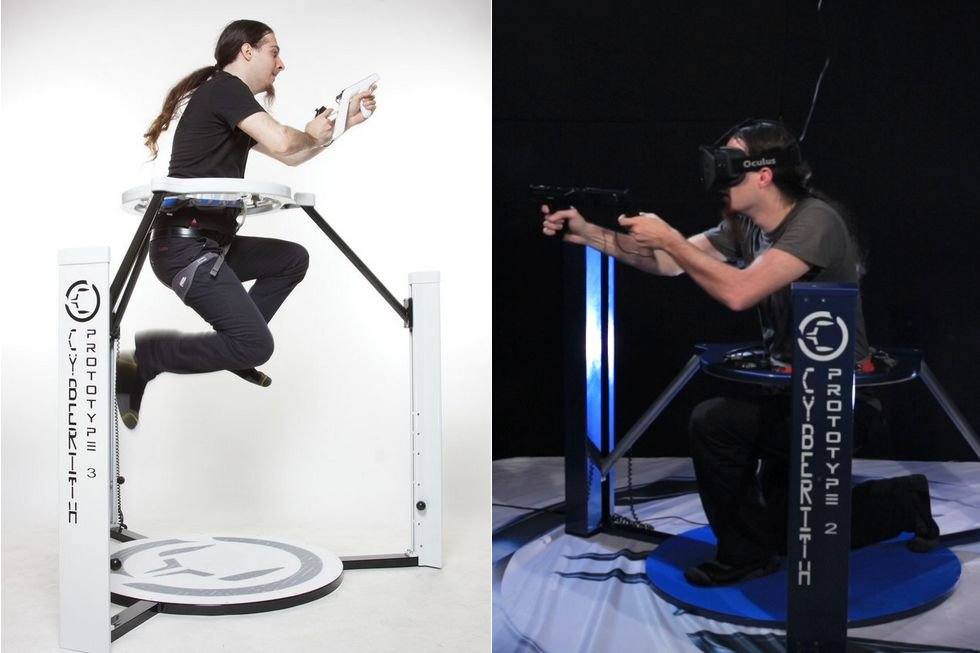
\includegraphics[width=0.9\linewidth]{./figures/ch3/cyberith_virtualizer}}
    \caption{}
    \label{Fig:cyverith_virtualizer}
  % \hspace{0.3cm}
  \end{subfigure}
  \begin{subfigure}{.5\textwidth}
  \centering
  {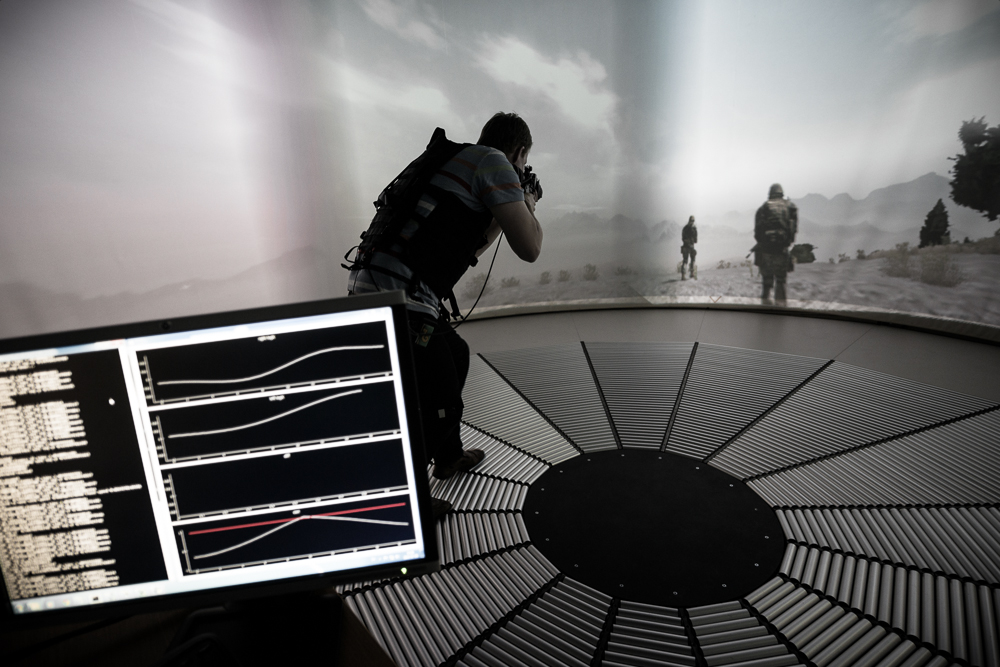
\includegraphics[width=0.9\linewidth]{./figures/ch3/omnideck}}
    \caption{}
    \label{Fig:omnideck}
  \hspace{0.3cm}
  \end{subfigure}
  \caption{\it (a) Tapis roulant multidirectionnel statique (\textit{Cyberith Virtualizer}) permettant de reconnaître, en plus de la marche et la course, des mouvements verticaux comme le saut ou l'accroupissement.
  (b) Premier tapis roulant multidirectionnel large et statique (\textit{Omnifinity Omnideck}), utilisé en couplage avec une technologie de \textit{tracking} optique afin de garantir un suivi précis des mouvements de l'utilisateur.
  }
  % \hspace{0.3cm}
\end{figure}

La technologie du \textit{tracking} optique joue également un rôle important puisqu'elle permet une certaine liberté de mouvement à l'utilisateur. En plus de profiter des espaces d'évolution larges qu'offrent les systèmes CAVE ou de murs d'écrans, les solution de \textit{tracking} permettent une implication plus importante du système vestibulaire de l'utilisateur et ainsi réduisent la décorrélation entre le déplacement virtuel et le déplacement ou mouvement réel. Cette réduction entraîne en parallèle une réduction importante du \textit{cybersickness} et constitue donc une alternative pertinente pour la navigation en RV.

\subsubsection{Paradigmes de navigation dans des scènes virtuelles réalistes}

Au delà des dispositifs et systèmes permettant la navigation, les paradigmes permettant de traduire une action dans le monde réel par un déplacement dans le monde virtuel sont nombreux. Ils ont été optimisé par les professionnels du jeu vidéo ou de la simulation professionnelle pour citer les plus actifs et ont permis de mettre au point des méthodes de navigation optimisées pour des contenus spécifiques et souvent réalistes.

Parmi les paradigmes de navigation s'appuyant sur le \textit{tracking} de tête ou du corps, on retrouve plusieurs approches: certaines considèrent chaque position de l'utilisateur par rapport à une zone spatiale de référence. Un déplacement dans la direction de la droite reliant la zone de référence à la position de l'utilisateur, à la manière d'un joystick où l'utilisateur serait le sommet du manche et la zone de référence constituerait la base de ce manche (voir Figure \ref{Fig:HCNAV}).

%\begin{figure}[h]
%  \centering
%  {\includegraphics[width=0.8\linewidth]{./figures/ch3/HCNAV}}
%    \caption{\it Exemple de l'utilisateur des déplacements relatifs d'un utilisateur par rapport à une zone de référence pour contrôler son déplacement dans le monde virtuel. L'orientation de son regard décidera également des rotations dans le monde virtuel. Il est donc possible d'avoir un contrôle de 6 degrés de liberté pour la navigation (3 en translation et 3 en rotation).}
%    \label{Fig:HCNAV}
%  \hspace{0.3cm}
%\end{figure}

Le \textit{tracking} des mouvements de l'utilisateur peuvent permettre de traduire le mouvement naturel de la marche en un équivalent dans le monde virtuel. La \textbf{marche redirigée} permet par exemple de reporter une marche en ligne droite dans le monde virtuel alors que la marche dans le monde réel est légèrement contrainte afin de ne pas sortir de l'aire de l'expérience.

Les paradigmes propres aux simulation de transports comme le vol ou la conduite de véhicule sont utilisés dans les scènes virtuelles constituées de grandes étendues à explorer (cf Figure \ref{Fig:driving_simu}). Proches des conditions réelles de pilotage ou de conduite, ils permettent d'assurer une certaine unicité de l'expérience réelle/virtuelle et possède une courbe d'apprentissage courte puisque basée sur l'expérience des utilisateurs.

Il existe donc une large variété de paradigmes permettant l'exploration et la navigation au sein de scènes écologiques. 

\begin{figure}[h]
  \begin{subfigure}{.5\textwidth}
  \centering
  {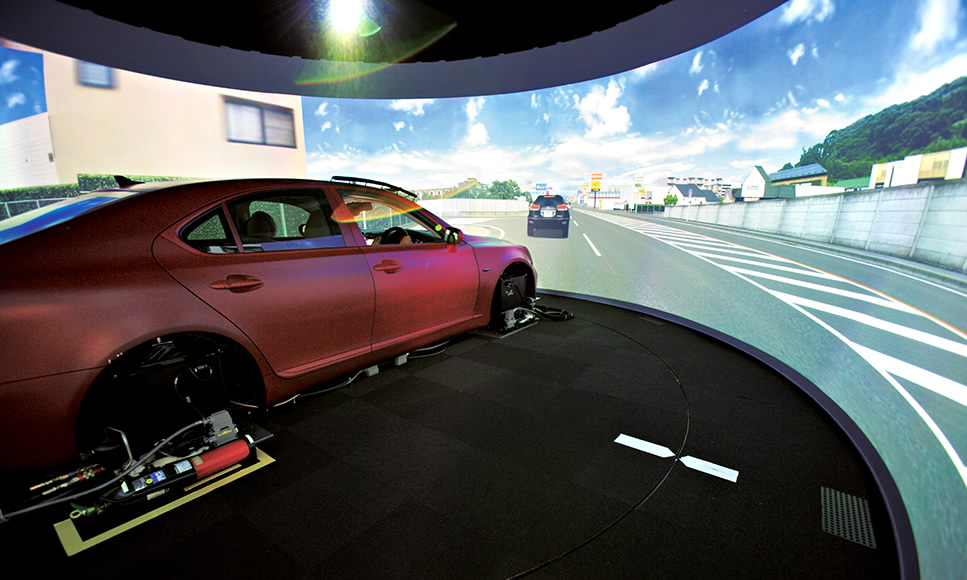
\includegraphics[width=0.9\linewidth]{./figures/ch3/driving_simu}}
    \caption{}
    \label{Fig:driving_simu}
  % \hspace{0.3cm}
  \end{subfigure}
  \begin{subfigure}{.5\textwidth}
  \centering
  {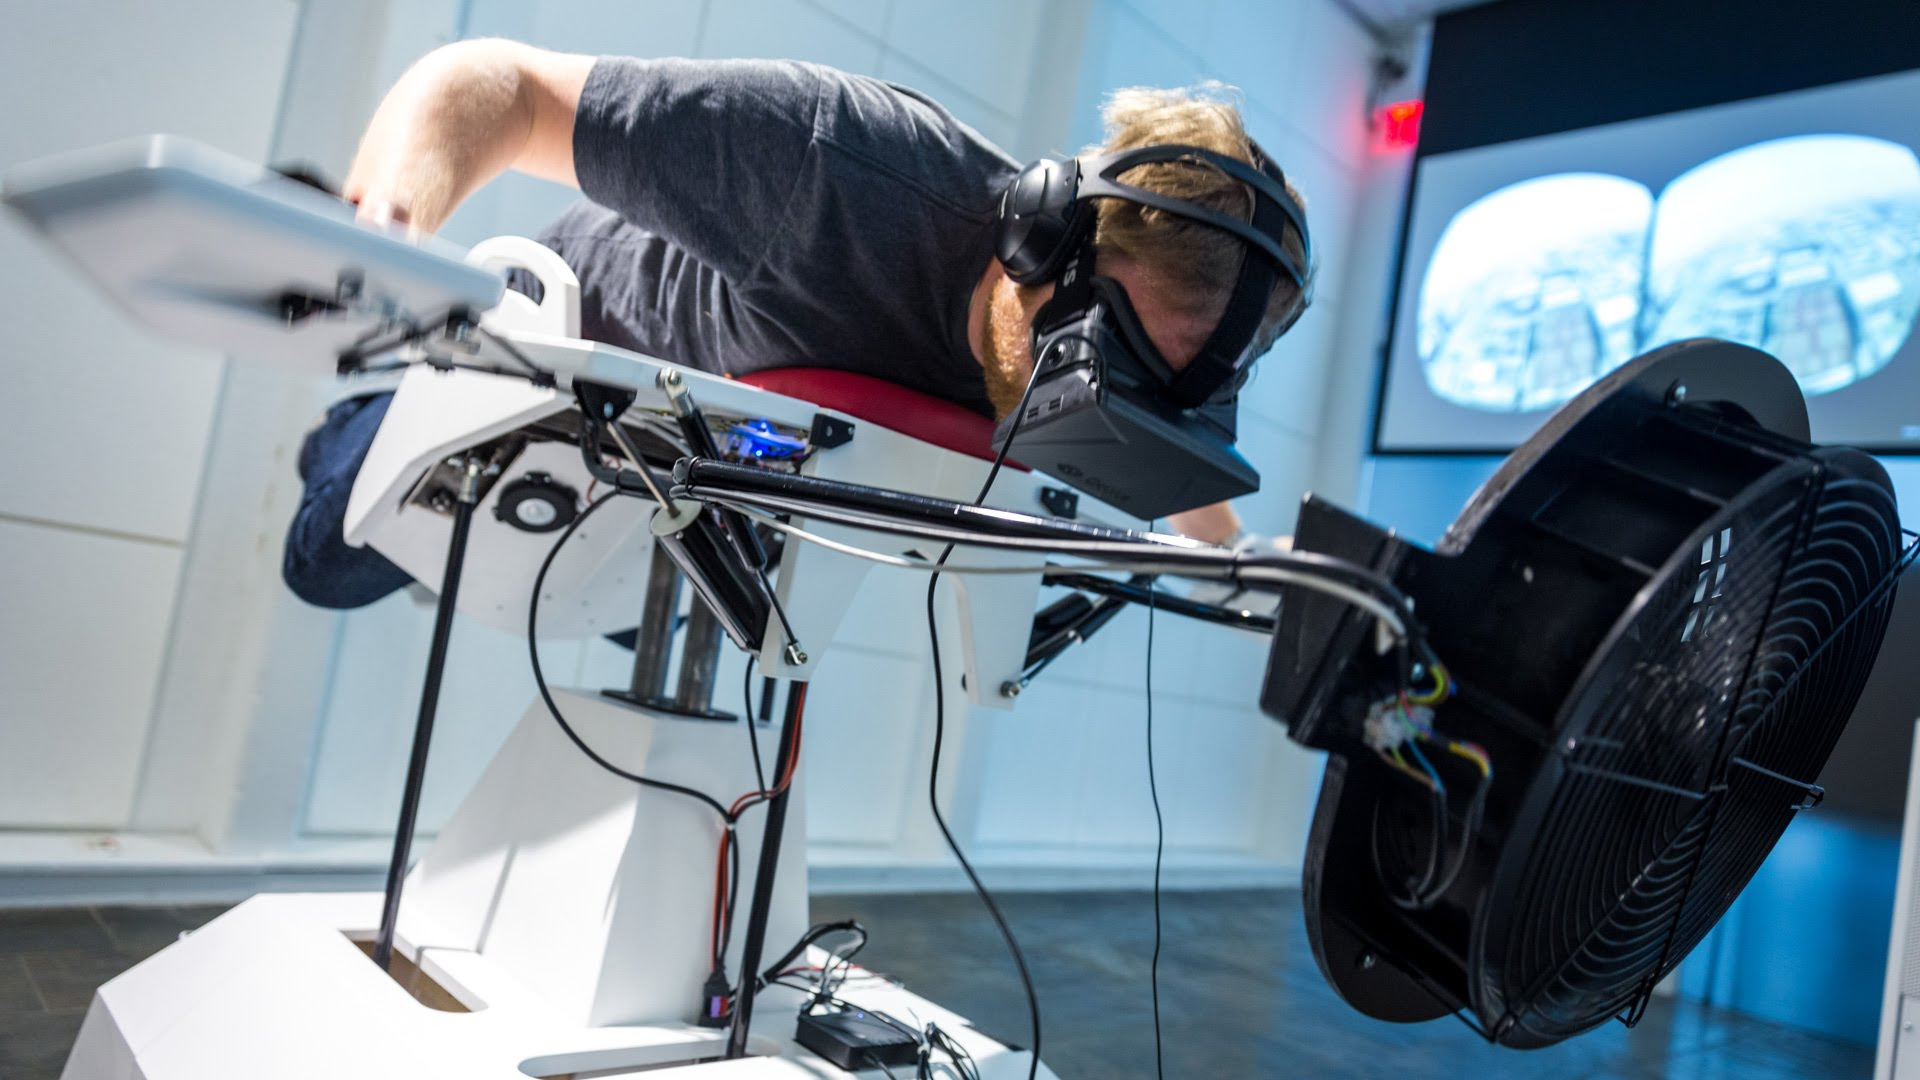
\includegraphics[width=0.9\linewidth]{./figures/ch3/flight_simu}}
    \caption{}
    \label{Fig:flight_simu}
  \hspace{0.3cm}
  \end{subfigure}
  \caption{\it (a) Exemple d'un simulateur de vol où les déplacements virtuels sont la conséquences des mouvements réels de l'utilisateur adoptant une posture de chute libre.
  (b) Simulateur de conduite dans un système de rétroprojection sur écran courbé.
  }
  % \hspace{0.3cm}
\end{figure}

\subsection{Méthodes de navigation dans des scènes virtuelles abstraites}

Conçus autour de contenus réalistes, les paradigmes cités précédemment sont néanmoins transposables à l'identique dans des scènes abstraites. Leur efficacité est cependant limitée du fait de la nature très différentes des données à observer. Alors que la navigation aura tendance à permettre l'exploration d'une surface virtuelle horizontale relativement étendue dans des scènes réalistes, les scènes abstraites scientifiques, et plus particulièrement les scènes moléculaires, concentrent les informations dans une zone centrale autour de laquelle l'utilisateur va évoluer. L'échelle de visualisation des données est capable d'augmenter la distance (toujours à l'échelle) des données observées mais la nature même de l'exploration est souvent différente. Sheidermann décrit la visualisation de données comme un processus où l'exploration est l'étape préliminaire avant les étapes de zoom et de filtre qui précèdent elle-même l'étape finale de l'obtention des détails à la demande \cite{shneiderman_eyes_1996}. Les différentes échelles de précision mises en avant dans cette description sont rarement retrouvées dans les paradigmes de navigation au sein de scènes virtuelles réalistes.

Bien qu'il existe de nombreux portages de logiciels experts de visualisation moléculaire dans des EV, la navigation au sein de données scientifiques dans ces derniers s’inspire encore largement de la manipulation d'objet retrouvé dans les logiciels de visualisation moléculaire courants (voir Figure \ref{Fig:pymol_nav}). La manipulation d'objets n'est cependant pas adaptée aux environnements virtuels. Le nombre et la complexité des tâches de manipulation sont trop nombreuses pour s'adapter aux EV 3d qui favorisent des paradigmes de navigation simplifiées. La taille des objets, dont l'ordre de grandeur est ramené à la taille humaine pour une meilleure immersion, est un second frein à l'approche par manipulation. Elle favorise en effet la perte du peu de repères spatiaux que pouvaient posséder l'utilisateur, ces repères étant souvent limités au seul objet intérêt, l'environnement (skybox, paysage, etc.) étant majoritairement vide (voir \ref{}).   

\begin{figure}[h]
  \begin{subfigure}{.5\textwidth}
  \centering
  {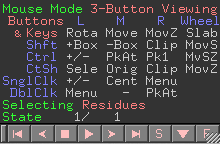
\includegraphics[width=0.9\linewidth]{./figures/ch3/pymol_nav}}
  % \hspace{0.3cm}
  \caption{}
  \label{Fig:pymol_nav}
  \end{subfigure}
  \begin{subfigure}{.5\textwidth}
  \centering
  {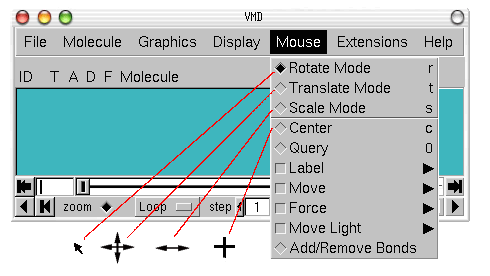
\includegraphics[width=0.9\linewidth]{./figures/ch3/vmd_nav}}
  \hspace{0.3cm}
  \label{Fig:vmd_nav}
  \end{subfigure}
  \caption{\it Capture d'écran des interfaces de manipulation offerts par PyMol (à gauche) et VMD à droite. Ils sont constitués de nombreuses combinaisons souris/clavier pour permettre d'utiliser l'ensemble des possibilités de manipulation disponibles.
  }
  % \hspace{0.3cm}
\end{figure}

Les seules tâches de navigation pouvant être identifiées au sein de logiciels experts de visualisation moléculaire se rapporte à des transitions progressives permettant de rejoindre une position spécifique depuis la position actuelle de l'utilisateur. Enfin, ces logiciels ne présentent aucune adaptation de la manipulation suivant le type de molécule observé et les paradigmes mis en jeu sont les mêmes que l'objet observé soit une protéine de quelques acides aminés ou bien un virus de plusieurs millions d'atomes. Dans tous les cas ils permettent une navigation totalement libre autour de la molécule et n'imposent aucune contrainte, au détriment de la conscience spatiale de l'utilisateur.

\section{Nouveaux paradigmes pour la RV}

Nous avons mis en évidence le besoin de mettre en place des paradigmes de navigation qui répondent aux problématiques posées par la visualisation moléculaire qui met en jeu des objets scientifiques abstraits, de plus en plus complexes, dans des environnements présentant un nombre réduit de repères spatiaux pour l'utilisateur.

Une piste de réflexion étudiée pour faire du processus de navigation un processus intuitif pour l'utilisateur est de le rendre cohérent avec les données qu'il observe. Si la trajectoire suivie par un utilisateur durant son exploration possède des échos dans la nature même de ce qu'il voit, alors nous parvenons à fournir une information pendant que l'utilisateur effectue une simple tâche de navigation. A l'image de ce qui a été fait pour les scènes réalistes, il est donc important de prendre en compte le contenu virtuel à explorer pour mettre en place un paradigme de navigation efficace. De la même façon, la navigation étant le support d'un nombre important de tâches en visualisation moléculaire, il nous a paru important de prendre également en compte l'activité des experts. 

Il nous a donc paru nécessaire et évident d'utiliser à la fois le contenu moléculaire et la tâche des experts pour guider les paradigmes de navigation. Ce travail a pu être fait en collaboration avec des biologistes travaillant sur des exemples concrets de modélisation de phénomènes biologiques précis et utilisant l'outil de la visualisation moléculaire quotidiennement. Il fut également possible de travailler pendant quelques temps avec des ergonomistes dont les approches d'analyses et de recueil des informations furent très utiles à l'identification des besoins des experts. Il est en effet important d'associer les experts du domaine aux étapes initiales de conception de paradigmes afin d'éviter un écart trop important entre leurs attentes et le résultat final.
Nous avons finalement, à la fin d'un premier processus de développement logiciel, mis en place un modèle de tâche sous la forme d'une décomposition hiérarchique en utilisant la méthodologie de \textit{Hierarchical Task Analysis} (HTA) afin d'évaluer la performance de nos paradigmes de navigation par rapport à une navigation libre effectuée en conditions d'immersion.

\subsection{Symétrie moléculaire et axes remarquables comme ancrage visuel}

Même si non-exclusif, notre attention fut rapidement portée sur les molécules les plus difficiles à visualiser ou manipuler dans les logiciels de visualisation moléculaire, à savoir les complexes moléculaires de grande taille. Ces complexes moléculaires sont souvent le résultat d'agencements de monomères (chaînes d'acide-aminés répétées) créant des multimères de taille importante et souvent constitués de plusieurs domaines. Les progrès des simulations moléculaires permettent désormais de simuler ces complexes moléculaires au sein de leur environnement, à l'image des protéines transmembranaires et des membranes dans lesquelles elles sont enfouies. Ces systèmes de plusieurs centaines de milliers d'atomes demandent donc une représentation et une navigation adaptées ne modifiant pas leur perception.

Ces assemblages moléculaires ont comme point commun la présence quasi systématique d'axes ou de centres de symétrie autour desquels ils sont construits. Or la symétrie est une particularité géométrique pouvant être facilement exploitable pour la mise en place de chemins de navigation optimisés. Mais ce n'est pas le seul avantage. Il est important de noter qu'au-delà de l'avantage conceptuel qu'ont ces symétries, elles possèdent également un rôle primordial dans la fonction même des complexes moléculaires \cite{goodsell_structural_2000}. Plusieurs exemples de d'arrangements symétriques trouvés dans des complexes biologiques sont illustrés dans la Figure \ref{}.
Ces axes de symétrie, obtenus de façon automatisés ou renseignés manuellement, peuvent donc permettre de définir une orientation fixe de la scène virtuelle moléculaire ainsi qu'être la base de la génération automatique de chemins de navigation. Les guides de navigation ne sont pas limités aux seules protéines symétriques et il est également possible d'identifier des axes principaux d'inertie qui pourront être utilisé de la même manière que les axes de symétrie. Il nous parait enfin important de permettre aux scientifiques de définir eux-mêmes les axes qu'ils considèrent comme important au sein de leurs complexes moléculaires, à l'image des membranes, de pores au sein des protéines ou de formes rectilignes.

\subsection{Contributions pour la représentation spatiale}

L'un des principaux avantages résultant de la réorientation possible d'une scène virtuelle est la fusion de l'axe de symétrie et du vecteur \textit{up} de la scène virtuelle. Un schéma rapportant les notions d'orientation à la fois de la scène virtuelle et de la caméra (ou de l'utilisateur puisqu'ils sont considérés comme fusionnés) est fournie dans la Figure \ref{}. 
Bien que sommaire, ce réarrangement permet de fournir un premier repère spatial fixe à l'utilisateur. Pour qu'il soit considéré comme tel tout au long de l'expérience virtuelle, nous contraignons le complexe moléculaire à garder cette orientation à tout instant. L'utilisateur est ainsi maintenu orienté de façon cohérente par rapport à l'objet d'étude à tout moment. Pour accroître l'apport spatial de cette réorientation, nous avons choisi d'ajouter une \textit{skybox} entourant la protéine. Une skybox est une texture fixe, présente tout autour de la scène virtuelle et jouant de rôle de paysage visuel non interactif (cf. Figure \ref). Le choix de la skybox doit respecter un certain nombre de pré-requis afin de remplir complètement son rôle \cite{vinson_design_1999}, ici de permettre à l'utilisateur de s'orienter à tout instant en regardant autour de lui. La skybox sélectionnée doit comporter deux parties supérieures et inférieures distinctes qui correspondrait à la partie haute et la partie basse de la molécule après sa réorientation. Elle peut très bien remplacer un environnement moléculaire (une membrane typiquement)non explicite et absente du modèle 3d observé.

\subsection{Exploration guidée}

De nombreux indices et informations peuvent être récoltés à partir des vues externes d'un complexe moléculaire. Nous savons que la forme générale d'une protéine peut fournir des indices importants sur son état fonctionnel. Nous avons également mis en avant dans la section \ref{visu_molecular} que certaines propriétés physico-chimiques ou géométriques comme la polarité, l'accessibilité au solvant ou l'intégration au sein de l'environnement peuvent être obtenues à partir d'une exploration succinte d'un complexe. Souvent associée au premières étapes de la visualisation, comme énoncé par Shneidermann \cite{shneiderman_eyes_1996}, l'exploration passe par un parcours extérieur du complexe observé. Nous avons mis en place des chemins de navigations circulaires autour de la molécule d'intérêt afin qu'une simple décision de l'utilisateur d'aller à sa droite ou à sa gauche lui permette de tourner autour de la molécule. Cela répond à une première difficulté qui est le suivi d'une trajectoire circulaire lorsque aucune contrainte n'est donnée à l'utilisateur. Il est souvent complexe de gérer des trajectoires circulaires lorsque seuls les axes de translations usuels sont contrôlés par l'utilisateur. Le déplacement latéral est ainsi géré automatiquement de façon à effectuer une rotation axiale autour de l'axe de symétrie, l'utilisateur peut néanmoins contrôler son déplacement vertical et sa distance à la molécule le long respectivement des axes \textit{up} et \textit{forward} de la caméra.

Tout au long du déplacement de l'utilisateur, son orientation est maintenue de façon à avoir le haut de la molécule pointant vers le haut de la scène virtuelle et inversement. Pour ce faire, le vecteur \textit{up} de la caméra est maintenu parallèle au vecteur \textit{up} de la scène. Le maintien de cette orientation est malheureusement préjudiciable lorsque l'utilisateur atteint la hauteur des extrémités hautes et basses du complexe observé. Nous avons donc mis en place un calcul de chemins inspiré de modèle de vecteur global \cite{khan_hovercam:_2005}. Ce modèle de vecteur garde le vecteur \textit{up} coplanaire à l'axe de symétrie et recalcule l'orientation de la caméra (vecteur \textit{forward}) à chaque pas jusqu'à atteindre une perpendicularité entre le vecteur \textit{up} et l'axe de symétrie lorsque l'utilisateur à atteint la hauteur maximale possible (voir Figure \ref{}).

Durant l'étape d'exploration externe l'utilisateur possède donc 3 degrés de liberté en translation même si le déplacement latéral le long du vecteur \textit{right} est contraint pour assurer un mouvement circulaire et le déplacement vertical le long du vecteur \textit{up} est contraint aux extrémités supérieures et inférieures de la protéine afin de garder le focus sur celle-ci. En terme de rotation, le seul degré de liberté autorisé est celui lié au tracking de tête qui verra la caméra suivre la direction du regard de l'utilisateur. Il n'est cependant pas possible de changer l'orientation explicitement pendant l'exploration sous contrainte.

La transition entre une exploration interne et externe d'un complexe moléculaire est une question importante qu'il ne semble pas possible de résoudre de façon simple et directe. Certains complexes moléculaires présentent des pores ou des structures centrales ayant un rôle prépondérant dans leur fonction. Parmi ces fonctions, le passage d'ions ou de molécules d'eau ou la liaison avec un ligand sont des phénomènes pouvant prendre place dans des régions enfouies dans un complexe moléculaire. Etant donné leur importance, il était nécessaire de réfléchir à des paradigmes de navigation efficaces dans ces zones d'intérêt tout en gardant la possibilité d'y effectuer des tâches complexes. Dans cette optique, nous avons mis en place la possibilité d'effectuer une transition automatique entre l'extérieur et l'intérieur d'un complexe. A la demande de l'utilisateur, un chemin de navigation rectiligne est calculé pour rejoindre l'intérieur du complexe. Ce chemin part de la position extérieure actuelle de l'utilisateur et rejoint le point de projection de sa position sur l'axe de symétrie de façon à ce que l'axe de symétrie et la trajectoire du chemin créé soient perpendiculaires. 

Lorsque l'intérieur d'une protéine est atteinte, un nouveau set de chemins de navigation est proposé afin de monter ou descendre dans le complexe le long de l'axe de symétrie. Dans ce mode de navigation, un seul degré de liberté en translation est possible ainsi qu'un seul degré de rotation, autour du vecteur \textit{up} de la caméra, comme si l'utilisateur tournait sur lui-même en gardant sa position, comme s'il se trouvait dans un ascenseur panoramique et qu'il dirigeait sa trajectoire verticale. Il est cependant possible d'alterner, pour la translation, vers un déplacement toujours le long de l'axe mais orienté de façon à être face aux extrémités de l'axe de symétrie. A la manière de l'exploration d'un tunnel, ce dernier représentant notre axe de symétrie, l'utilisateur sera capable d'avancer ou de reculer dans ce tunnel. Il pourra de nouveau tourner sur de lui même autour du vecteur \textit{up} de la caméra.

\subsection{Optimisation du parcours des régions répétées}

La symétrie, et plus généralement l'agencement des monomères d'un complexe moléculaire, induit souvent l'apparition d'événements structuraux comme la liaison d'un ligand, l'ouverture d'une poche de liaison ou la simple variation structurelle d'une région de façon répétée pour chaque monomère identique. Ainsi, la liaison d'un ligand sur une première chaîne A signifiera certainement que ce ligand peut aussi se lier à une chaîne identique B, C, D, etc. Comparer ces régions d'intérêts est très utile pour détecter d'éventuels comportements asynchrones ou des effets différents, il peut par contre être difficile de naviguer d'une région à une autre pour effectuer cette comparaison. Grâce à la symétrie, il nous a été possible de mettre en place un mode de navigation adapté à cette problématique permettant d'automatiser complètement le passage d'une région d'intérêt à la région répétée sur un autre monomère. Ce calcul est rendu possible par l'utilisation de l'axe de symétrie comme axe de rotation pour la caméra dont l'angle de rotation sera simplement dépendant de l'angle de rotation ayant été calculé entre les monomères. Un assemblage standard verra cet angle être de 360 degrés divisé par le nombre de monomères identiques du complexe. Il est cependant également possible d'utiliser des scripts de calcul plus fins afin d'obtenir les valeurs d'angle précises entre les monomères impliqués. Lorsque cette information est connue (elle est par défaut calculée lors de la phase d'initialisation de la scène virtuelle) et que l'utilisateur a choisi son point de vue sur la région d'intérêt, alors une simple interaction avec un bouton permet de parcourir les différents monomères, préservant le point de vue choisi initialement. Il est possible de parcourir les monomères dans les deux sens. Chaque déplacement est effectué automatiquement et une série d'interpolations au cours de la trajectoire de la caméra permet une transition douce entre les différentes positions.

\subsection{Trouver un point de vue optimal}

Même si l'exploration peut apporter un grand nombre d'informations, certains phénomènes moléculaires ne concerne qu'une poignée d'atomes ou de résidus. Au sein de large structures de plusieurs millions d'atomes, ces zones d'intérêt deviennent difficiles à visualiser à cause de la densité des particules voisines. De plus, certaines régions sont profondément enfouies dans le complexe moléculaire, transformant la simple tâche de visualisation en un défi pour l'utilisateur. Afin de résoudre cette problématique, nous avons développé un algorithme capable de calculer le meilleur point de vue pour la caméra, connaissant les coordonnées de la cible et la distance à laquelle la caméra devra être située. Cet algorithme prend en compte les atomes entourant la cible et calcule les cônes de vue les plus larges pour identifier le meilleur point de vue. L'utilisateur aura la possibilité de choisir entre plusieurs cônes de vue afin d'obtenir un angle de vue différent sur la cible choisie.

\subsubsection{Algorithme}

L'algorithme utilisé pour obtenir les cônes de vue peut être décomposé de la sorte:

\begin{enumerate}
	\item L'utilisateur fournit les coordonnées 3d de la cible soit en entrant les valeurs (x,y,z) au sein d'une fenêtre de saisie, soit via une sélection directe. Si la cible comporte plus d'un atome alors les coordonnées du centre de masse de la sélection seront calculées. La hauteur désirée du cône de vue \textit{d} est également demandée, elle correspondra à la distance de la caméra par rapport à la cible.
	\item Tous les atomes situés au sein d'une sphère de rayon \textit{d} et centré sur les coordonnées de la cible sont considérés comme voisins et comme potentielles occlusions, ou obstacles, pour le cône de vue. Leurs coordonnées 3d sont stockées.
	\item L'ensemble des coordonnées 3d des atomes voisins stockés précédemment sont décalés dans l'espace d'un vecteur correspondant aux coordonnées 3d de la cible (un cible située en $(1.2,-9.2,5.5)$ entraînera un décalage des coordonnées de $\overrightarrow{(1.2,-9.2,5.5)}$). Cela entraîne la création d'une sphère dont les coordonnées d'atomes sont centrées autour d'une origine (la cible) située en $(0,0,0)$.
	\item L'ensemble des coordonnées cartésiennes des atomes contenus dans la sphère sont transformées en coordonnées sphériques. Les coordonnées sphériques sont composées de 3 paramètres: une distance radiale à l'origine \textit{r}, un angle polaire $\theta$ (theta) et un azimuth $\phi$ (phi). En mettant de côté la distance radiale, nous obtenons pour chaque atome une information de direction par rapport à l'origine donnée par les angles $\theta$ et $\phi$. Il est possible de fixer la distance radiale de tous les atomes voisins à la valeur de \textit{d} et ainsi mettre en place une projection de ces atomes sur la sphère de rayon \textit{d}. Lorsque la projection est effectuée, la recherche du plus large cône de vue passera par la recherche du plus grand cercle vide à la surface de la sphère. Le concept est illustré dans la Figure \ref{}
	\item Puisque la valeur de la distance radiale est identique pour l'ensemble des atomes voisins, il est possible de créer un nuage de point correspondant aux valeurs de $\phi$ en fonction des valeurs des valeurs de $\theta$ afin d'obtenir une représentation aplatie de la surface de la sphère en 2d contenant l'ensemble des points projetés (un point = un atome). La matrice 2d ainsi obtenue est étendue de 50\% le long des ordonnées et des abscisses afin de prendre en compte la périodicité de la sphère. Il n'est pas nécessaire de l'étendre au-delà de 50\% puisque la taille maximum d'un cercle vide sera la taille du plus long côté de la matrice. Si aucune extension n'est effectuée, nous pourrions manquer les solutions qui apparaîtraient à l'extrémité de la matrice où deux régions de la sphère aplatie se rejoindraient. Nous pouvons d'ailleurs voir dans la Figure \ref{} que l'absence d'extensions nous auraient fait manquer deux solutions. Pour synthétiser, ces nuages de points 2d peuvent être considérés comme une carte 2d de la distribution à la surface de la sphère des atomes ayant été projetés.
	\item A partir de la liste des atomes formés par les paires $\theta$/$\phi$, un diagramme de Voronoi est calculé. Nous obtenons une liste de sommets de Voronoi associés chacun à un triplet des trois atomes les plus proches.
	\item La distance entre chaque sommet de Voronoi et les trois points les plus proches est calculée et les plus grandes valeurs de cette distance indiquera les plus grands cercles vides présents sur la surface de la sphère. Ces cercles auront pour centre un sommet de Voronoi et passeront obligatoirement par les trois points les plus proches puisque l'algorithme de Voronoi impose que chaque sommet soit équidistant d'au moins 3 points, ceux-ci étant également les plus proches. Le cercle avec le rayon le plus large sera considéré comme le cercle vide le plus grand (cf. Figure \ref{}). Il est important de noter que, en dépit de l'extension de la matrice, nous ne sélectionnons pas de centres de cercles situés à l'extérieur de la boîte entourant les premières coordonnées sphériques tracées (en pointillé dans la Figure \ref{}) et correspondant aux extensions. Cependant les points appartenant au cercle peuvent eux se situer dans les parties étendues du graphe.
	\item Les valeurs $\theta$/$\phi$ du centre des plus larges cercles vides sont transformés en coordonnées cartésiennes et décalés de nouveau d'un vecteur opposé à celui utilisé pour le premier décalage (avec notre exemple ce vecteur serait $\overrightarrow{(-1.2,9.2,-5.5)}$). Le rayon des cercles donne un angle d'ouverture qui sera utilisé par la suite pour calculé une trajectoire optimale (voir ci-dessous).
	\item Les coordonnées cartésiennes peuvent ensuite être choisies itérativement par l'utilisateur pour se positionner par rapport à la cible, la caméra sera contrainte de façon à toujours faire face à la cible.
\end{enumerate}

Cet algorithme a une complexité faible en $\theta(n.\log{n})$ (avec $n$ désignant le nombre d'atomes) puisque la recherche des voisins de la cible est calculée en $n$-1 itérations (constant) et que le diagramme de Voronoi et la recherche du cercle le plus large est effectué en $\theta(n.\log{n})$ dans le pire des cas où tous les atomes du système sont considérés comme voisins et situés dans la sphère de rayon \textit{d}. L'algorithme est capable de fournir une liste des vues les plus dégagées sur une cible de façon quasi instantanée et donc permet à l'utilisateur de changer de point de vue rapidement.

\subsubsection{Atteindre les points de vue optimaux}

La recherche d'un point de vue optimal peut être effectuée sur n'importe quelle région du complexe moléculaire étudié, nous avons cependant mis en avant son apport dans le cas de régions d'intérêt à observer enfouies dans le complexe et très difficilement atteignables. Le chemin entre la position d'un utilisateur au moment où il décide de rentrer dans un mode de recherche de point de vue optimal et la position optimale trouvée passe souvent par le passage au travers du complexe, dans des régions potentiellement denses en atomes et perturbantes pour le point de vue de l'utilisateur. Il nous a donc paru nécessaire de mettre en application les recommandations énoncées dans la section \ref{cybersickness} qui rappelaient l'importance des transitions entre points de vue pour diriger une trajectoire entre deux points d'une scène virtuelle. Afin tout d'abord de minimiser l'impact négatif que pourrait avoir ce déplacement sur l'utilisateur et ensuite pour permettre à l'utilisateur de garder une conscience spatiale de l'environnement pendant le déplacement et ainsi pouvoir se situer rapidement lors de son positionnement final devant la cible visée.
Une transition progressive et automatique est ainsi mise en place. Pour calculer les différents points du chemin reliant la position initiale de l'utilisateur à la position optimale de visualisation de sa cible, l'algorithme développé précédemment est utilisé de façon répété à différentes valeurs de \textit{d} et appliqué à une aire restreinte de la surface de la sphère correspondant aux aires délimitées par les cercles vides identifiés lors de la première itération de l'algorithme. Comme illustré dans la Figure \ref{} nous obtenons un chemin de navigation avec le moins d'occlusions pendant la majorité de la phase d'approche de la position optimale.

Cela permet également de laisser à l'utilisateur la possibilité de choisir entre la position offrant le plus large cône de vue sur la cible ou la position dont le chemin d'accès est le plus dégagé parmi les positions optimales recensées. Selon la distance entre la position initiale de l'utilisateur et les positions optimales identifiées, la première partie de la trajectoire peut être calculé comme une ligne droite afin de réduire le nombre d'itérations de l'algorithme, ce dernier demandant en plus un temps de calcul augmentant à chaque pas de temps à cause de la taille de la sphère créée et du nombre de voisins considérés.

Le passage d'un point de vue optimal à un autre est quant à lui simplement le fruit de techniques d'interpolation classiques prenant en compte la préservation du focus sur la cible, la recherche d'une orientation de la caméra dont le vecteur \textit{up} est le plus parallèle possible de l'axe de symétrie et le chemin le plus court pour atteindre la nouvelle position.

\subsubsection{Grande densité atomique}

Dans le cas de régions très denses et d'une cible particulièrement enfouie dans ces régions, nous avons ajouté la possibilité de rendre transparents les atomes situés entre la caméra et la cible. Ce traitement graphique n'est pas effectué dans l'intégralité de l'écran mais seulement dans un cercle de taille fixe centré sur le centre de l'écran. Cela permet de supprimer toute occlusion le long du déplacement pour atteindre le point de vue optimal désiré.

Dans le cas où l'algorithme de point de vue optimal n'est pas suffisant pour permettre la visualisation d'une cible sans occlusions devant la caméra, nous avons mis en place une étape supplémentaire dans le processus de visualisation. Cette étape est une étape de modification structurelle du complexe moléculaire. Elle consiste à découper le complexe moléculaire en sous-régions distinctes et de permettre leur dissociation pendant l'exploration. Ce découpage ne peut cependant pas se faire de façon simpliste et demande une définition intelligente des sous-régions afin de ne pas perdre toute cohérence structurale et donc biologique du complexe moléculaire. Nous avons de nouveau utilisé la géométrie du complexe moléculaire comme base de décision pour ce découpage. Puisque la symétrie définie les monomères d'un complexe, nous pouvons facilement découper la structure pour que ces monomères puisse bouger de façon contrôlée et de manière à ne pas perdre la forme générale de la structure (voir Figure \ref{}). L'utilisateur a de plus la possibilité, à chaque instant, d'étendre, rétrécir ou simplement déplacer les monomères du complexe en fonction de l'axe ou du centre de symétrie qu'il choisit (dans le cas où plusieurs axes/centres ont été renseignés). Un mode automatisé a également été ajouté permettant d'étendre ou rétrécir la structure suivant la position de l'utilisateur par rapport au complexe. Une distance maximum d'extension peut être imposée afin de préserver les informations d'interaction entre les monomères ou les sous-unités découpées. Cette adaptation structurelle permet la mise en lumière des interfaces enfouies entre les sous-unités et permettre de calculer de nouveaux points de vue optimaux. Pour éviter toute surcharge dans le processus de modification structurelle, la configuration spatiale initiale du complexe peut être retrouvée à chaque instant.

\subsubsection{Evaluation par Analyse Hiérarchique de la Tâche (HTA)}

L'arbre de tâche HTA est présenté dans la Figure \ref{} et décrit la manière de répondre à une tâche courante de visualisation moléculaire, la recherche des acides aminés impliqués dans une liaison avec un ligand selon les monomères envisagés. Ce modèle a été extrait grâce aux experts du domaine et donne une subdivision progressive de la tâche énoncée. Les subdivisions les plus externes pouvant finalement être évaluées d'un point de vue temporel et ainsi permettre une approximation de la durée de la tâche suivant un set de conditions particulier. Ici nous comparons des conditions de navigation libres avec des conditions de navigation guidée utilisant les paradigmes expliqués précédemment. Nous ferons l'hypothèse d'une
\\
\\
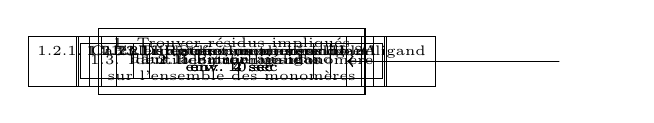
\begin{tikzpicture}
\tikzset{grow'=right,level distance=120pt}
\tikzset{execute at begin node=\strut}
\tikzset{every tree node/.style={anchor=base west}}
\Tree 
 [.\node[draw, font=\tiny, align=center]{1. Trouver résidus impliqués \\dans la liaison au ligand \\sur l'ensemble des monomères};
    [.\node[draw, font=\tiny, align=center]{1.1. Situer ligand} ;
        [.\node[draw, font=\tiny, align=center](start){1.1.1. Sélectionner ligand \\env. 2 sec}; ]
        [.\node[draw, font=\tiny, align=center]{1.1.2. Déplacer camera vers ligand \\env. 10 sec}; ] ]
    [.\node[draw, font=\tiny, align=center]{1.2. Identifier résidus} ;
        [.\node[draw, font=\tiny, align=center]{1.2.1. Calculer distance entre résidus et ligand \\env. 10 sec}; ]
        [.\node[draw, font=\tiny, align=center]{1.2.2. Lister résidus a moins de 2A \\env. 2 sec}; ] ]
    [.\node[draw, font=\tiny, align=center]{1.3. Identifier prochain monomère};
    	[.\node[draw, font=\tiny, align=center]{1.3.1. Retour vue d'ensemble \\env. 4 sec}; ]
    	[.\node[draw, font=\tiny, align=center](end){1.3.2. Identifier monomère cible \\env. 4 sec}; ] ] 
    ] 
 \draw[semithick,->] (end)..controls +(east:5) and +(east:5)..(start);
    \\           
\end{tikzpicture}
\\
\\
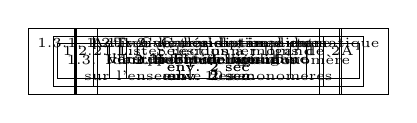
\begin{tikzpicture}
\tikzset{grow'=right,level distance=150pt}
\tikzset{execute at begin node=\strut}
\tikzset{every tree node/.style={anchor=base west}}
\Tree 
 [.\node[draw, font=\tiny, align=center]{1. Trouver résidus impliques \\dans la liaison au ligand \\sur l'ensemble des monomeres};
    [.\node[draw, font=\tiny, align=center]{1.1. Situer ligand} ;
        [.\node[draw, font=\tiny, align=center]{1.1.1. Sélectionner ligand \\ env. 2 sec}; ]
        [.\node[draw, font=\tiny, align=center]{1.1.2. Calcul optimal du\\ point de vue \\ env. 2 sec}; ] ]
    [.\node[draw, font=\tiny, align=center]{1.2. Identifier résidus} ;
        [.\node[draw, font=\tiny, align=center]{1.2.1. Calculer distance entre \\résidus et ligand \\ env. 10 sec}; ]
        [.\node[draw, font=\tiny, align=center]{1.2.2. Lister résidus à moins de 2A \\ env. 2 sec}; ] ]
    [.\node[draw, font=\tiny, align=center]{1.3. Identifier prochain monomère};
    	[.\node[draw, font=\tiny, align=center]{1.3.1. Activer la translation automatique \\ vers prochain monomère \\ env. 2 sec}; ] ] ] \\           
\end{tikzpicture}
\\

Nous avons identifié une tâche métier type consistant à identifier, au sein d'un complexe protéique multimérique composé de 5 monomères, les différents acides aminés impliqués dans la liaison avec un ligand particulier pour chaque monomère du complexe. Nous utiliserons l'exemple de la liaison du bromoforme avec GLIC pour illustrer cet exemple. Cette tâche est divisable en trois étapes principales: Recherche du ligand dans un monomère, l'identification des résidus en interaction, accès au monomère suivant. Suivant les conditions d'expérience initiales, la subdivision de chacune de ces trois étapes est différente et décrite dans les deux arbres hiérarchiques précédents. On obtient un temps d’exécution pour cette tâche plus élevé dans les conditions normales (environ 2 min 32 s) que dans les conditions intégrant nos paradigmes de navigation (environ 1 min 28 s). L'accès à la cible (ici le ligand) et la recherche du monomère suivant sont les deux étapes cruciales où les paradigmes de navigation permettent un gain de temps substantiel. De façon moins tangible car difficilement mesurable, nos paradigmes permettent également d'assurer une vision claire de la zone cible et donc pourrait être considéré comme facilitant l'étape 1.3.

\subsection{Conclusion et perspectives}

La visualisation de données est un processus analytique où l'observation et l'exploration des données amènent de nouvelles informations au scientifique. Cette information peut être acquise d'une façon active, en mesurant par exemple la distance entre deux atomes, ou de façon passive, en se déplaçant et en observant des phénomènes qui ne peuvent être que partiellement décrits par des valeurs brutes. C'est le cas par exemple de la forme des surfaces situées à l'interface entre deux partenaires biologiques se liant entre-eux qui ne peuvent être définis que de manière parcellaire par des propriétés d'hydrophobicité, d'accessibilité au solvant ou de volumee et qui nécessitent donc d'être visualisés afin d'être totalement comprises. L'acquisition d'informations passe donc par un processus de navigation qui dirige l'utilisateur vers les événements qu'il désire observer ou vers des régions avec lesquelles il désire interagir. La navigation est un processus important en immersion car il peut décider du confort de l'utilisateur pour effectuer ses tâches, passives ou actives. Le malaise du virtuel, lié en partie à la perte de repères spatiaux est un phénomène qu'il est important de prendre en compte mais qui fut absent des approches de navigation, et  plus précisément de manipulation, développées avec les logiciels experts de visualisation moléculaire. Cette absence est principalement due à l'aspect négligeable du cybersickness en conditions non-immersives.

Fort du constat de l'absence de développements de navigation spécifiques à la visualisation de données scientifiques et plus particulièrement moléculaires, nous avons proposé plusieurs paradigmes ou modes de navigation pouvant répondre à ce besoin. Nos efforts se sont portés sur l'utilisation de l'objet d'intérêt, ici un complexe moléculaire, comme base intelligente et dynamique de la créations de chemins de navigation contraints, semi-automatisés ou automatisés suivant les modes de navigation considérés. Notre approche peut s'inscrire dans le processus de visualisation de données évoqué par Shneidermann et introduisant une échelle de granularité partant de l'exploration globale des données à l'observation précise de certains phénomènes ponctuels et locaux.

Une étape supplémentaire dans notre approche et dans le développement de notre set de paradigmes serait d'accorder une plus grande importance à l'utilisateur pour décider des patterns et des structures qui définiraient les chemins de navigation calculés. Il nous semble important d'utiliser l'expertise scientifique afin de créer des paradigmes de navigation répondant à des besoins spécifiques pouvant varier suivant la nature du complexe moléculaire étudié. Ce plus haut niveau d'interaction ne doit pourtant pas dépasser le niveau d'implication cognitive que doit comporter la navigation, cette dernière restant bien souvent un moyen d'accéder à d'autres tâches plus complexes et nécessitant davantage de réflexion de la part de l'utilisateur. Et même si les études ont montré qu'une augmentation de la charge cognitive est une bonne manière de réduire le \textit{cybersickness} (voir section \ref{cybersickness}) elle peut également réduire l'efficacité des tâches annexes au processus de navigation.

Des méthodes ergonomiques comme la HTA nous ont permis de mettre en évidence les apports en terme de performance et de simplification des processus de nos paradigmes de navigation.

Le retour d'expérience des utilisateurs d'un logiciel est important mais néanmoins souvent oublié quand on arrive aux étapes de post-développement. Avec l'évolution rapide des techniques, plateformes et approches de visualisation, il est important de revoir les nouveaux besoins des experts et les nouvelles possibilités offertes par les nouvelles technologies. 





